\section{API-Service}

Bei HTTP-Anfragen können Inhalte in der Anfrage als verschiedene Typen übergeben werden.
Hier wird der Typ \verb|mutltipart/forma-data| verwendet.
Bei diesem Typ können sowohl Text als auch Dateien übertragen werden.
Jeder Text oder jede Datei werden dabei als Wert betrachtet und müssen einen Schlüssel vergeben bekommen.
Das heißt, dass alle Informationen als Schlüssel-Wert-Paar an den API-Service gesendet werden.
Die Schlüssel, die verwendet werden sollen, werden wie folgt vergeben.
Die DatasourceDefinition bekommt den Schlüssel "`datasource-definition"'.
Der Wert dahinter kann entweder eine JSON-Datei oder ein JSON-Text sein.
Die Schlüssel der hochgeladenen Dateien sind frei wählbar.

Die DatasourceDefinition besteht zu Teilen aus Feldern, die automatisch durch die Services gefüllt werden.
Daher wird ein weiteres Datenmodell für die Eingabe von Informationen bei der REST-API benötigt.
Dafür wird die DatasourceDefinitionInput (\cref{fig:datasource-definition-input}) verwendet.
In diesem Modell befinden sich alle Felder, die durch den Benutzer befüllt werden können.
Aus den Daten dieses Modells erstellt der API-Service dann die Revisionen für die DatasourceDefinition.

\begin{figure}
    \centering
    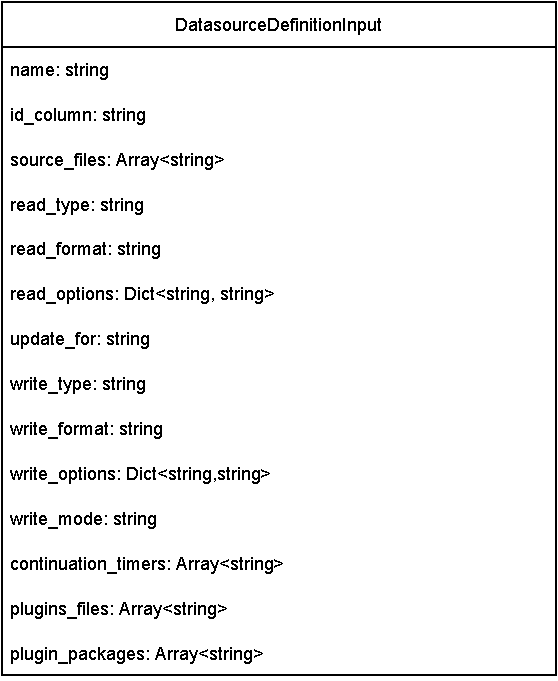
\includegraphics[width=.65\textwidth]{Grafiken/Umsetzung-Definition-Input.pdf}
    \caption{Felder Datenquellen-Eingabe}
    \label{fig:datasource-definition-input}
\end{figure}

\subsection{Hochladen von Dateien}

Für jede Datenquelle können Quell- oder Plugin-Dateien hochgeladen werden.
Um eine hochgeladene Datei in der Datenquelle auch zu verwenden, muss der Schlüssel unter dem die Datei hochgeladen wird in der entsprechenden Liste entweder unter "`source\_files"' oder unter "`plugin\_files"' hinzugefügt werden.
Alternativ können auch die Namen unter denen bereits Dateien für die Datenquelle gespeichert wurden in die Listen eingefügt werden.

Bei der Verarbeitung der Eingabe prüft der API-Service für jeden Eintrag der Listen, ob eine Datei mit diesem Schlüssel hochgeladen wurde.
Ist das der Fall, wird die entsprechende Datei in das HDFS hochgeladen.
Der Name, unter dem die Datei gespeichert wird, setzt sich aus der Nummer der Revision, dem vergebenen Schlüssel und der Endung der Datei zusammen.
Lädt man also eine bei der ersten Erstellung einer DatasourceDefinition eine Datei "`data.json"' mit den Schlüssel "`file"' hoch, wird diese als "`r000\_file.json"' im "`sources"'-Ordner der DarasourceDefinition gespeichert.
Analog werden Plugin-Dateien genau so behandelt.

Wenn keine Datei in der Anfrage gefunden wurde, wird geschaut ob im HDFS eine Datei mit dem Namen existiert.
Wird eine Datei gefunden, wird der Name an die neue Revision angehangen.
Es ist wichtig zu beachten, dass alle Dateien der alten Revision, die nicht explizit in einer der Listen angegeben werden, nicht in der neuen Revision verwendet werden.
Sie bleiben jedoch gespeichert und können später wieder hinzugefügt werden.
Da die Dateien nach den Datenquellen aufgeteilt sind, ist es aktuell nicht möglich Plugins oder Quell-Dateien in anderen Datenquellen wieder zu verwenden.
Hier müsste man die Datei für jede Datenquelle hochladen.
